\section{Methodology}

In this chapter, I will explain the methodology used in this research to build and evaluate depression severity classifiers. It includes some final data preparation steps such as label encoding, sampling and data augmentation strategies, describes the pipelines used for model training and evaluation strategies.

To begin the modeling process, I divided the final dataset into train and test subsets, with a split ratio of 80 to 20. Given the small amount of data, I experimented with a 70-30 split initially, but the differences between the splits were insignificant.

Since this task is multi-label classification instead of binary, I used the label encoder from the Scikit-learn library to encode string class labels into integer format. The encoder was then fit on the training labels and then applied to both training and test labels for consistency.

For evaluating model performance, I used a 5-fold cross-validation using StratifiedKFold. This approach is quite standard, but it is especially important to preserve the relative frequency of each class in every fold, given the class imbalance in my dataset. Similarly, I experimented with a 10-fold cross-validation, but the differences were minimal.

The first operation that I implemented to mitigate the impact of class imbalance was to compute class weights. I then applied those class weights to all compatible classifiers to adjust the learning process so that underrepresented classes receive proportionally more attention.

\subsection{Machine Learning Methodology}

In this part of the research, I evaluated both traditional machine learning models and sentence embedding-based classifiers, using two types of feature representations: Term Frequency-Inverse Document Frequency (TF-IDF) vectors and sentence embeddings. My previous research in this domain concluded that TF-IDF is superior to the Bag-of-Words(BoW) approach, so I chose this as traditional feature representation.

I configured the TF-IDF vectorizer to use unigrams and bigrams with a maximum of 5,000 features and filtered out the extreme common and rare terms to reduce noise. For the sentence embeddings, I utilized the all-MiniLM-L6-v2 model to compute dense vector embeddings of the input text. This approach should capture contextual and semantic relationships better than sparse representations.

The initial performances of the models were very poor, so I experimented with SMOTE (Synthetic Minority Oversampling Technique) to oversample the minority class in the training set. I applied SMOTE separately to both TF-IDF and embedding-based features.

I tested and evaluated three traditional classifiers across both feature types: Logistic Regression, Linear SVM and Random Forest. Each model was trained with the computed class weights and validated using the cross-validation strategy I mentioned earlier. For each model, I computed cross-validation scores and confusion matrices, and the main evaluation metrics are accuracy, F1 score, recall and precision, all weighted by class frequency.

After applying cross-validation, I compared all models based on their average performance across folds. The best-performing model will be re-trained on the full training set and evaluated on the testing set. 

\subsection{Deep Learning Methodology}

For the next component of my research, I implemented a Bidirectional Long Short-Term Memory (BiLSTM) neural network, enriched with two kinds of pre-trained GloVe embeddings that capture semantic meaning: general-domain embeddings and twitter-domain embeddings. My goal is to find out if the twitter-based embeddings will outperform the general-domain ones, given that they are trained specifically on social media texts, similar to my classification task.

I began by performing some data augmentation operations to further address the class imbalance. I applied a synonym-replacement augmentation approach using the nlpaug library with the SynonymAug augmenter configured with WordNet as the source. Each sample from the severe class was augmented with four additional variants, which boosted the minority class size. The original training size was 11,014 samples. The augmenter provided an additional 3,896 severe samples which produced 14,910 total training size post-augmentation.

After augmentation, I re-encoded the target labels and transformed them into categorical one-hot representations using TensorFlow, in order to make them compatible with the multi-class softmax output layer used in the neural networks.

The text sequences were tokenized with a vocabulary size limit of 10,000 and padded to a fixed maximum length of 100 tokens. I then mapped the 100-dimensional GloVe vectors to the tokenized vocabulary to create two embedding matrices, which I used as non-static input layers in their respective models.

I customized the model architecture as BiLSTM to capture both past and future temporal dependencies in the token sequences. The model layer architecture can be found in the figure below.

\begin{figure}
    \centering
    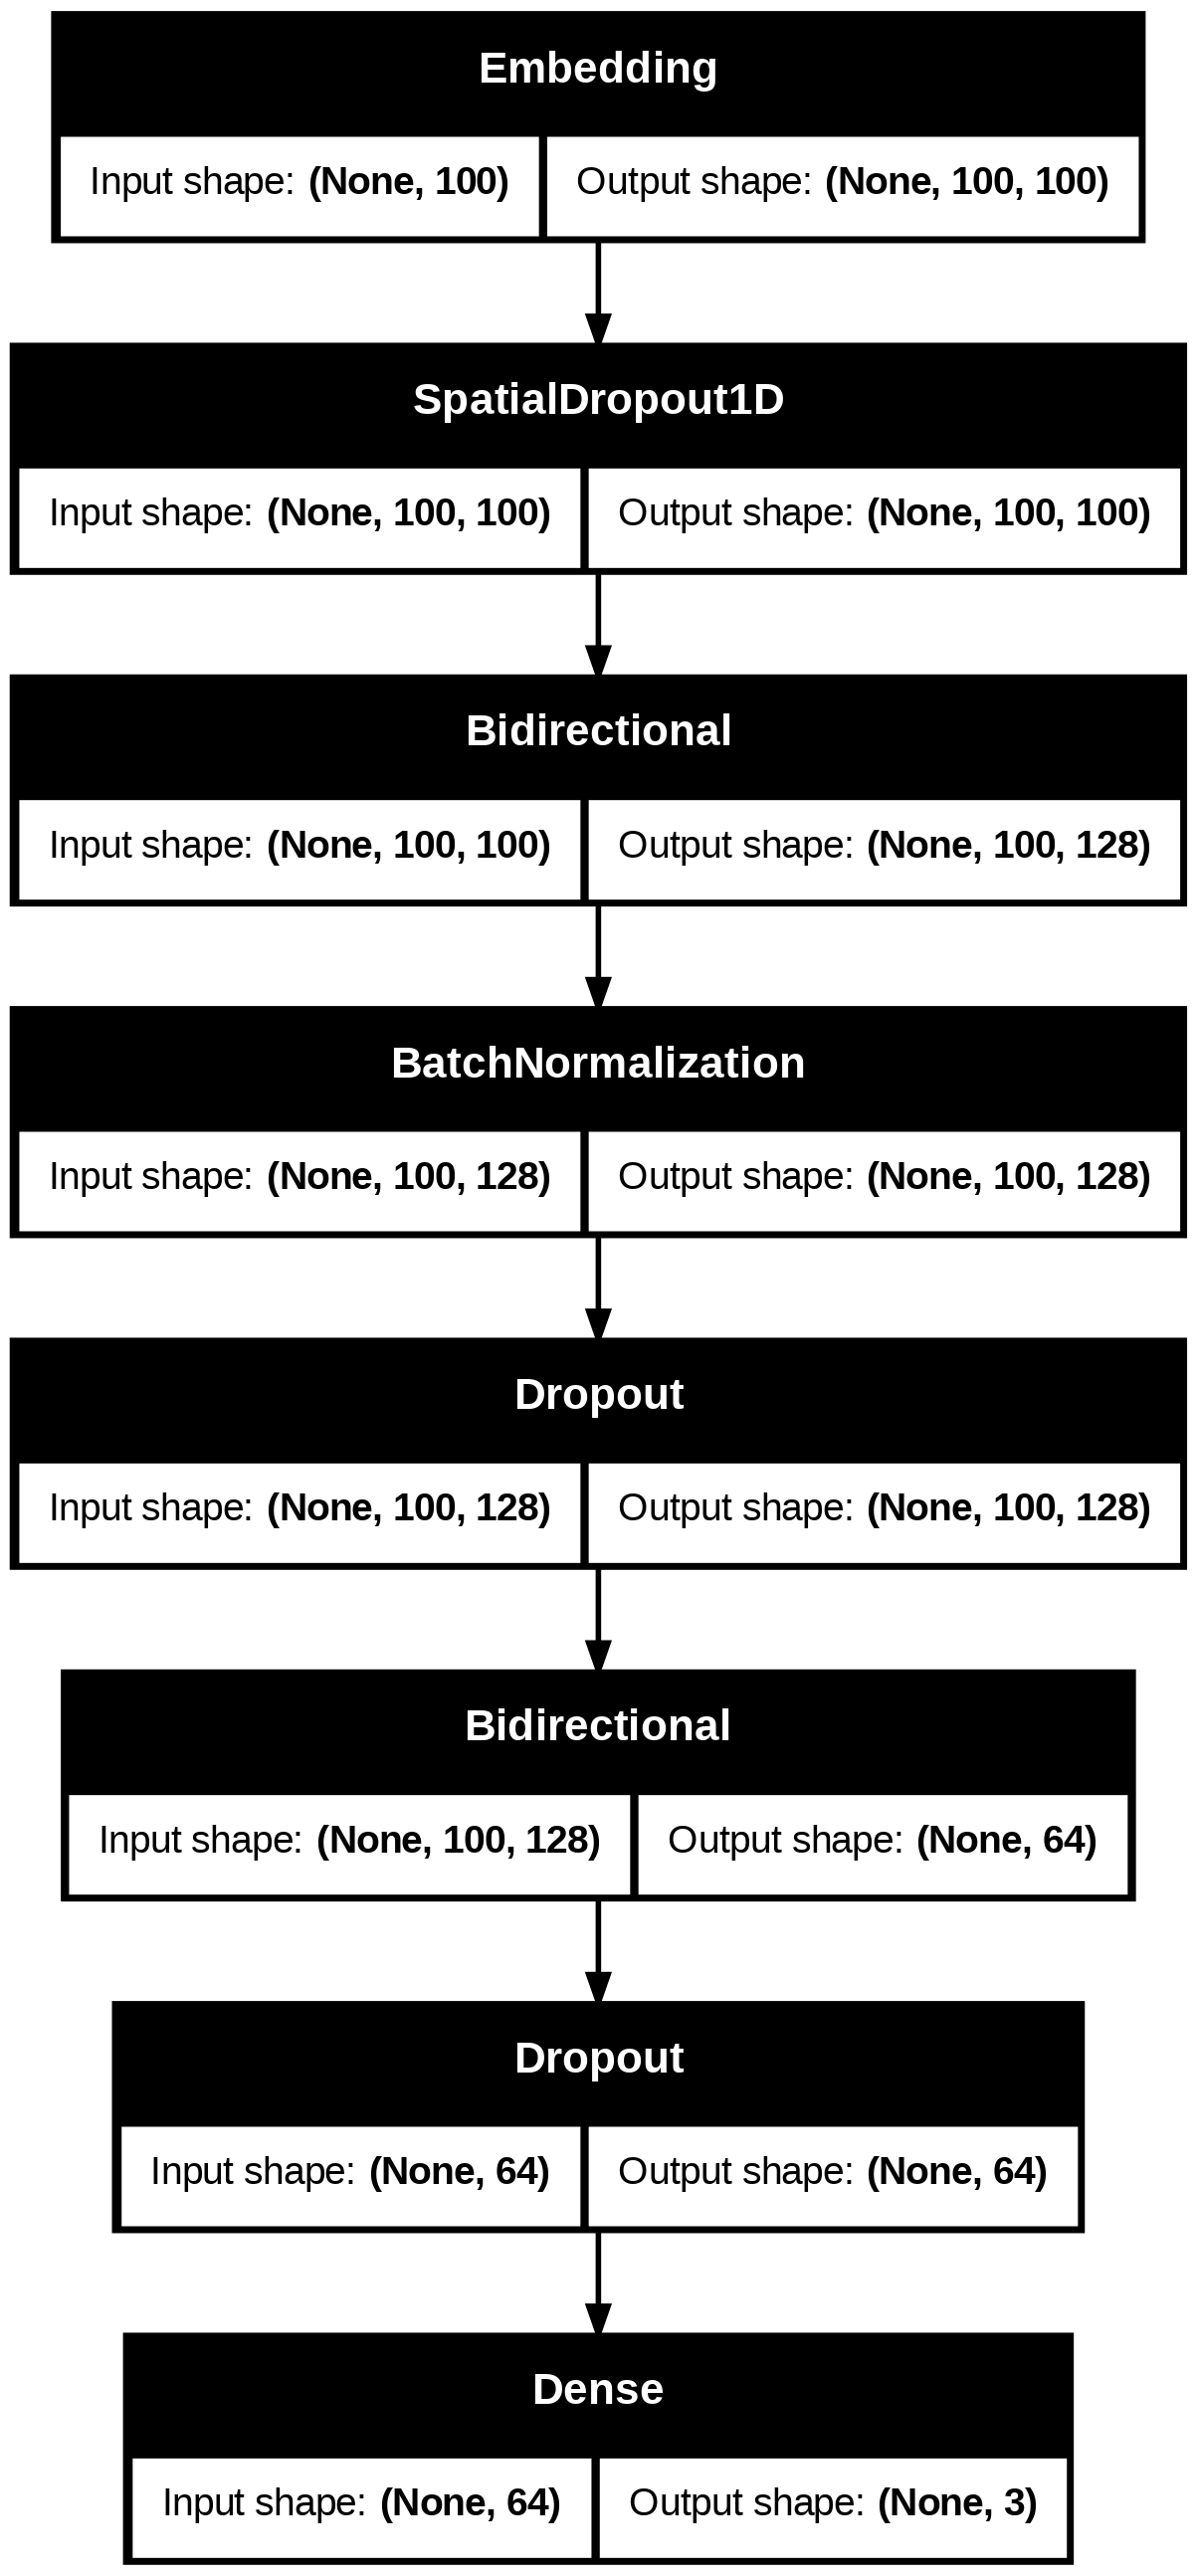
\includegraphics[width=0.5\linewidth]{img/model-architecture.png}
    \caption{BiLSTM Model Layer Architecture}
    \label{Fig_1}
\end{figure}

The initial Embedding layer is initialized with the appropriate pre-trained GloVe embedding and converts each token into a 100-dimensions vector. I also allowed for fine-tuning during training by specifying trainable weights.

I then used a Spatial Dropout layer of 0.2 to randomly drop entire embeddings, instead of individual features, in the hope of helping the model to generalize better.

Following that, I applied the first Bidirectional LSTM layer with 64 units to capture context in both forward and backward directions. This should enable the model to understand both preceding and succeeding context in sentences.

Initial training experiments were unstable, so I added a Batch Normalization layer that normalizes intermediate outputs and stabilizes training.

In order to help with generalization and prevent overfitting I also used three separate Dropout layers, with a rate of 0.2 and 0.5 respectively.

A second BiLSTM layer with 32 units was stacked next to allow the model to refine learned representations with additional processing.

The final layer is a standard Dense layer with a softmax activation and three output units, which corresponds to my three severity labels.

Each model was compiled with the Adam optimizer and trained using categorical cross-entropy loss. I implemented an early stopping callback to prevent overfitting based on a validation loss, with a patience of 3 epochs. I also applied the class weights from the original label distribution.

I trained each model up to 20 epochs with a batch size of 512 and then evaluated them on the test set using the classification metrics defined at the beginning of this chapter.

\subsection{LLM-based Methodology}

Another goal of this research is to compare the effectiveness of Large Language Models (LLMs) with traditional machine learning and deep learning models. For this, I implemented a two-stage transfer learning approach using DistilBERT.

I began by pre-training a DistilBERT model on an unlabeled corpus using Masked Language Modeling. This step aimed to adapt the general-purpose language model to the specific linguistic pattern found in my domain-related corpus. I used the uncased base version and trained for 3 epochs with a masked token probability of 15\% using the Trainer API from HuggingFace Transformers library.

After pre-training, I reused the masked language model to initialize DistilBERT for sequence classification with three output labels corresponding to my severity classes. I used for both steps the fast tokenizer with a maximum length of 128 tokens.

Finally, I fine-tuned the classification model using supervised learning for 6 epochs. I configured the training with a learning rate of $2 \times 10^{-5}$, a batch size of 32 and weight decay of 0.01.

After fine-tuning, I evaluated the model using custom metrics, including accuracy, precision, recall and F1-score.